\documentclass[12pt,a4paper]{article}
\usepackage[utf8]{inputenc}
\usepackage{amsmath}
\usepackage{amsfonts}
\usepackage{amssymb}
\usepackage{makeidx}
\usepackage{graphicx}
\usepackage{hyperref}
\usepackage{graphicx}
\usepackage{xcolor}


\hypersetup{
	colorlinks=true,
	linkcolor=blue,
	filecolor=magenta,      
	urlcolor=cyan,
}

\author{Aliaksandr Panko}

\title{Final Exam}
\begin{document}
	\maketitle
	\tableofcontents
\section{Task 1: Stationarity of L}
To check stationarity Augmented Dickey-Fuller test is used. HO - nonstationary(unit root exists)
\begin{verbatim}
adf_test <- tseries::adf.test(data.fe$L,alternative = 'stationary') 
print(adf_test)
\end{verbatim}
\begin{center}
	\makebox[\textwidth]{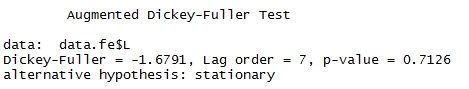
\includegraphics[width=390pt]{p1}}
\end{center}
Based on the test we cannot reject H0. This means that we assume that the data are not stationary.

Let's hava a look at the serias:
\begin{verbatim}
plot(data.fe$L, type = "l")
\end{verbatim}
\begin{center}
	\makebox[\textwidth]{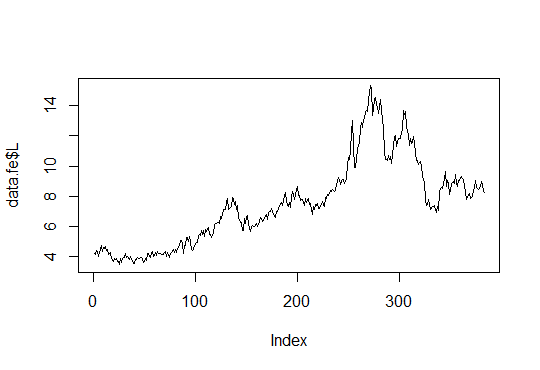
\includegraphics[width=390pt]{p2}}
\end{center}
We can clearly see two trends, which proves nonstationarity.

To continue we need to take differences:
Take differencies:

\begin{verbatim}
difL <- diff(data.fe$L)
plot(difL, type = "l")
\end{verbatim}
\begin{center}
	\makebox[\textwidth]{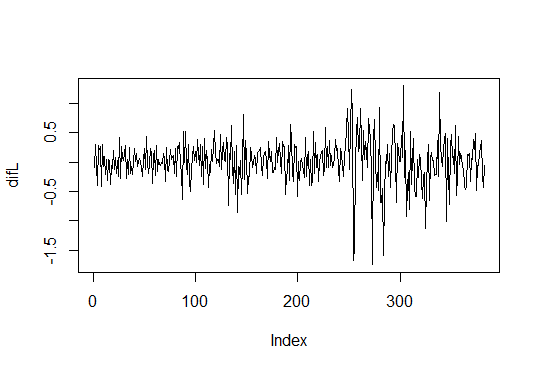
\includegraphics[width=390pt]{p3}}
\end{center}
Is looks much better.

Let's have a look at acf and pacf

\begin{verbatim}
acf(difL)
pacf(difL)
\end{verbatim}
\begin{center}
	\makebox[\textwidth]{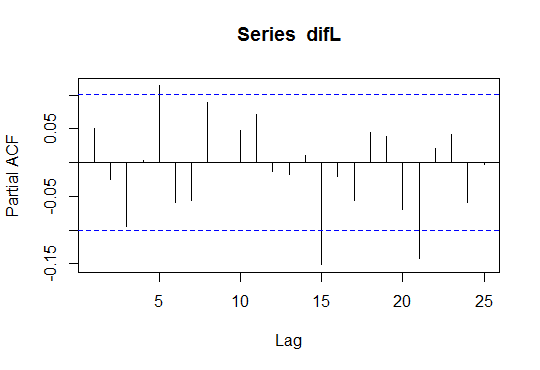
\includegraphics[width=390pt]{p4}}
\end{center}
\begin{center}
	\makebox[\textwidth]{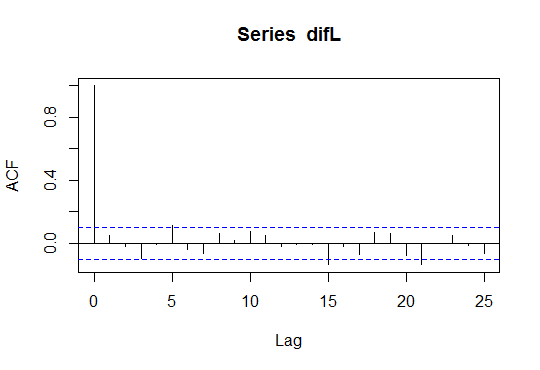
\includegraphics[width=390pt]{p5}}
\end{center}
Choose the best model automatically

\begin{verbatim}
forecast::auto.arima(difL, seasonal=FALSE)
\end{verbatim}
\begin{center}
	\makebox[\textwidth]{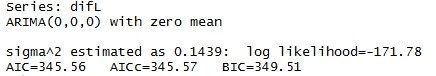
\includegraphics[width=390pt]{p6}}
\end{center}
The function gives us the same result as we could see ARIMA (0,0,0).
So, basically the difference of long run rates is noise.

\section{Task 2 : Model for a stock price index}
Firstly, we need to determine all regressors that could be important for the model since omitted regressors have critical impact.

In my opinion all of these factors are potentially possible, so I will use iterative process to eliminate insignificant ones.

So, initially use all the regressors to avoid ommited ones.

Since all questions are about returns we will derive returns from the price and work with them.

Calculate returns using price X

\begin{verbatim}
data.fe$returns = NA
for(i in 2:nrow(data.fe))
{
data.fe$returns[i] = (data.fe$X[i] - data.fe$X[i-1]) / data.fe$X[i-1]
}

plot(data.fe$returns, type = "l")
\end{verbatim}
\begin{center}
	\makebox[\textwidth]{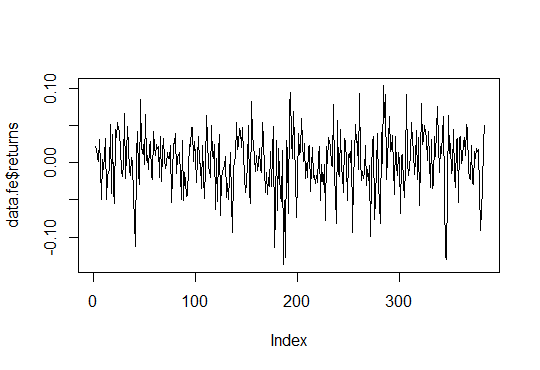
\includegraphics[width=390pt]{p7}}
\end{center}
Check Normal Distribution. H0 - distribution is normal
\begin{verbatim}
shapiro.test(data.fe$returns)
\end{verbatim}
\begin{center}
	\makebox[\textwidth]{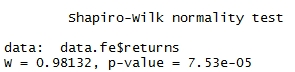
\includegraphics[width=390pt]{p8}}
\end{center}
\begin{verbatim}
hist(data.fe$returns)
\end{verbatim}
\begin{center}
	\makebox[\textwidth]{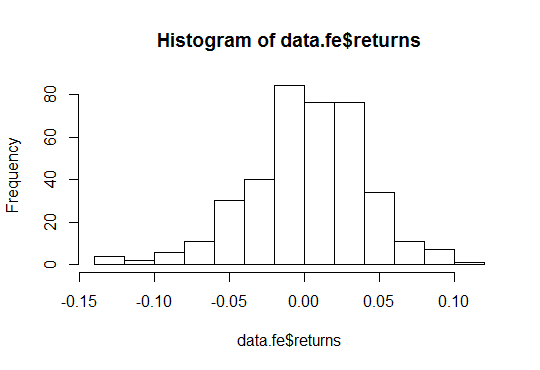
\includegraphics[width=390pt]{p9}}
\end{center}
We can see that they are skewed to the right.

So, we can see that returns are not normal.

Based on iterative elimination of regressors we have the next model:

\begin{verbatim}
	model = lm(data = data.fe, formula = data.fe$returns ~ data.fe$L +
	#data.fe$D +
	#data.fe$E +
	data.fe$C : data.fe$P +   
	data.fe$S)  
	summary(model)
\end{verbatim}
\begin{center}
	\makebox[\textwidth]{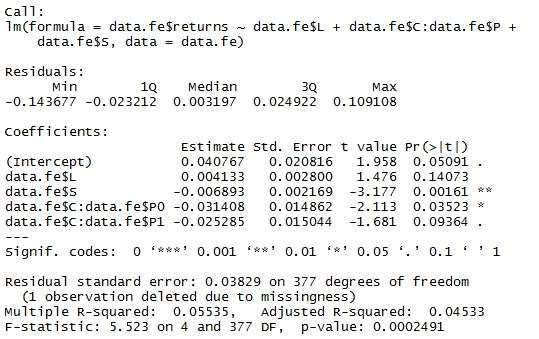
\includegraphics[width=390pt]{p10}}
\end{center}
The model is fairly bad wirh R\^2 only around 4\%

Let's execute Breusch-Pagan test to check the homoscedasticity: HO - homoscedasticity
\begin{verbatim}
	lmtest::bptest(model) 
\end{verbatim}
\begin{center}
	\makebox[\textwidth]{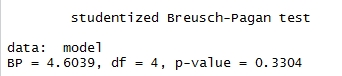
\includegraphics[width=390pt]{p11}}
\end{center}
We cannot reject H0 of homoscedasticity at 5\% level of significance

Check autocorrelation. HO - no autocorrelation
\begin{verbatim}
Box.test(resid(model1),type="Ljung",lag=20,fitdf=1)
\end{verbatim}
\begin{center}
	\makebox[\textwidth]{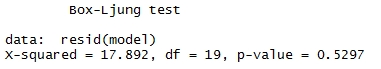
\includegraphics[width=390pt]{p12}}
\end{center}
The test says we don't have autocorelation here at 5\% level of significance

So the result is:
President is not significant and the claim from 3b is  not true too

\end{document}